\documentclass{article}

\usepackage{tikz}
\usepackage{amsmath, amssymb}
\usetikzlibrary{fit, positioning}
\usepackage{ragged2e}
\usepackage{ulem}


\newcommand{\bs}[1]{\boldsymbol{#1}}
\newcommand{\gs}[3]{\mathcal{N}(#1|#2,#3)}
\begin{document}

\begin{flushleft}


	% graphical model
	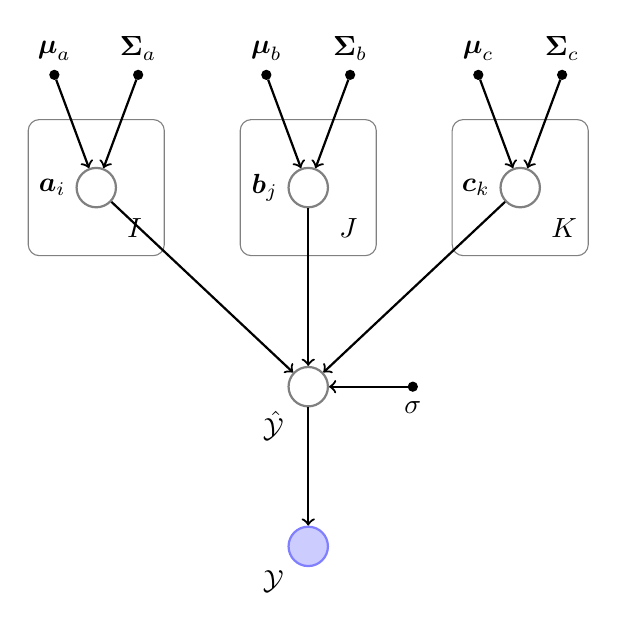
\begin{tikzpicture}
	% style
	[rounded corners,
	param/.style={circle,draw=black!100,fill=black!100,thick,inner sep=0pt, minimum size=1mm},
	visible/.style={circle,draw=blue!50,fill=blue!20,thick,inner sep=0pt,minimum size=5mm},
	hidden/.style={circle, draw=black!50, fill=white!100, thick, inner sep = 0pt, minimum size=5mm},
	plate/.style={rectangle, draw=black!50, inner sep=6mm},
	plate_label/.style={rectangle, inner sep = 0mm}]
	
	% matrix A
	\node [param] (mu_a) [label=above:$\bs{\mu}_a$]{};
	\node [hidden, node distance=1.2cm and 3mm] (a_i) [below right=of mu_a,label=left:$\bs{a}_i$]{};
	\node [param, node distance=1.2cm and 3mm] (sigma_a) [above right=of a_i, label=above:$\bs{\Sigma}_a$]{};
	\node [plate_label,fit=(a_i), label=below right:$I$] (plate_label_a) {};
	\node [plate, fit=(a_i)] (plate_a) {};

	% matrix B
	\node [param, node distance= 1.5cm] (mu_b) [right=of sigma_a,label=above:$\bs{\mu}_b$]{};
	\node [hidden, node distance=1.2cm and 3mm] (b_j) [below right=of mu_b,label=left:$\bs{b}_j$]{};
	\node [param, node distance=1.2cm and 3mm] (sigma_b) [above right=of b_j, label=above:$\bs{\Sigma}_b$]{};
	\node [plate_label,fit=(b_j), label=below right:$J$] (plate_label_b) {};
	\node [plate, fit=(b_j)] (plate_b) {};

	% matrix C
	\node [param, node distance= 1.5cm] (mu_c) [right=of sigma_b,label=above:$\bs{\mu}_c$]{};
	\node [hidden, node distance=1.2cm and 3mm] (c_k) [below right=of mu_c,label=left:$\bs{c}_k$]{};
	\node [param, node distance=1.2cm and 3mm] (sigma_c) [above right=of c_k, label=above:$\bs{\Sigma}_c$]{};
	\node [plate_label,fit=(c_k), label=below right:$K$] (plate_label_c) {};
	\node [plate, fit=(c_k)] (plate_c) {};
	
	% tensor
	\node [hidden, node distance=2cm] (Y') [below=of b_j, label=225:$\mathcal{\hat{Y}}$]{};
	\node [visible, node distance=1.5cm](Y) [below=of Y', label=225:$\mathcal{Y}$] {};
	%\node [hidden, node distance =1cm] (Z) [right=of X, label=right:$\mathcal{Z}$] {};
	\node [param, node distance=1cm] (sigma) [right=of Y', label=below:$\sigma$]{};
	\path[->,thick] (mu_a)		edge (a_i)
	                (sigma_a)	edge (a_i)
	                (mu_b)		edge (b_j)
	                (sigma_b)	edge (b_j)
	                (mu_c)		edge (c_k)
	                (sigma_c)	edge (c_k)
	                (a_i)		edge (Y')
	                (b_j)		edge (Y')
	                (c_k)		edge (Y')
	                (Y')			edge (Y)
	                (sigma)		edge (Y');
	                %(Z)			edge (X);
\end{tikzpicture}

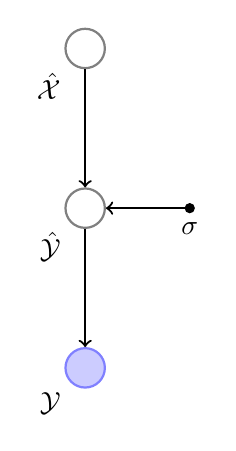
\begin{tikzpicture}
% style
	[rounded corners,
	param/.style={circle,draw=black!100,fill=black!100,thick,inner sep=0pt, minimum size=1mm},
	visible/.style={circle,draw=blue!50,fill=blue!20,thick,inner sep=0pt,minimum size=5mm},
	hidden/.style={circle, draw=black!50, fill=white!100, thick, inner sep = 0pt, minimum size=5mm},
	plate/.style={rectangle, draw=black!50, inner sep=6mm},
	plate_label/.style={rectangle, inner sep = 0mm}]
	
	% tensor
	\node [hidden](X') [label=225:$\mathcal{\hat{X}}$] {};
	\node [hidden, node distance=1.5cm] (Y') [below=of X', label=225:$\mathcal{\hat{Y}}$]{};
	\node [visible, node distance=1.5cm] (Y) [below=of Y', label=225:$\mathcal{Y}$] {};
	\node [param, node distance=1cm] (sigma) [right=of Y', label=below:$\sigma$]{};
	\path[->, thick] (X') edge (Y')
	                 (Y') edge (Y)
	                 (sigma) edge (Y');
\end{tikzpicture}

\section{probability Model}

According \textit{Canonical polyadic(CP) Tensor Fatorization}, the approximation of the tensor $\mathcal{X} \in \mathbb{R}^{N \times M \times L}$ of mode 3 is given by

\begin{equation}
	\mathcal{X} \approx \mathcal{\hat{X}} = \sum_{r=1}^{R}\bs{a}_{:,r}\circ\bs{b}{_:,r}\circ\bs{c}_{:,r}.
\end{equation}

Assuming that each $\bs{a}_i \in \mathbb{R}^{N \times 1}$ has a Gaussian distribution with a mean $\bs{\mu}_a \in \mathbb{R}^{N \times 1}$ and a covariance matrix $\bs{\Sigma}_a \in \mathbb{R}^{N \times N}$, the conditional distribution of $\bs{a}_i$ is 
\begin{equation}
	p(\bs{a}_i|\bs{\mu}_a,\bs{\Sigma}_a)=\mathcal{N}(\bs{a}_i|\bs{\mu}_a,\bs{\Sigma}_a).
\end{equation}
And the conjugate prior probability of $\bs{\mu}_a$ and $\bs{\Sigma}_a$ is
\begin{align}
	p(\bs{\mu}_a, \bs{\Sigma}_a) &= p(\bs{\Sigma}_a)p(\bs{\mu}_a|\bs{\Sigma}_A)=NIW(\bs{\mu}_a, \bs{\Sigma}_a|\bs{m}^a_0,\kappa^a_0,\nu^a_0,\bs{S}^a_0), \\
	p(\bs{\mu}_a|\bs{\Sigma}_a) &= \mathcal{N}(\bs{\mu}_a|\bs{m}^a_0, \frac{1}{\kappa^a_0}\bs{\Sigma}_a),\\
	p(\bs{\Sigma}_a) &= IW(\bs{\Sigma}_a|\nu^a_0, \bs{S}^a_0).
\end{align}
Similarly, for $\bs{b}_j \in \mathbb{R}^{M \times 1}$, we have
\begin{align}
p(\bs{b}_j|\bs{\mu}_b,\bs{\Sigma}_b)&=\mathcal{N}(\bs{b}_j|\bs{\mu}_b,\bs{\Sigma}_b)\\
p(\bs{\mu}_b, \bs{\Sigma}_b) &=NIW(\bs{\mu}_b, \bs{\Sigma}_b|\bs{m}^\beta_0,\kappa^\beta_0,\nu^\beta_0,\bs{S}^\beta_0), \\
	p(\bs{\mu}_b|\bs{\Sigma}_b) &= \mathcal{N}(\bs{\mu}_b|\bs{m}^\beta_0, \frac{1}{\kappa^\beta_0}\bs{\Sigma}_b),\\
	p(\bs{\Sigma}_b) &= IW(\bs{\Sigma}_b|\nu^\beta_0, \bs{S}^\beta_0),
\end{align}
and for $\bs{c}_k \in \mathbb{R}^{L \times 1}$, we have
\begin{align}
	p(\bs{c}_k|\bs{\mu}_c,\bs{\Sigma}_c)&=\mathcal{N}(\bs{c}_j|\bs{\mu}_c,\bs{\Sigma}_c)\\
p(\bs{\mu}_c, \bs{\Sigma}_c) &=NIW(\bs{\mu}_c, \bs{\Sigma}_c|\bs{m}^c_0,\kappa^c_0,\nu^c_0,\bs{S}^c_0), \\
	p(\bs{\mu}_c|\bs{\Sigma}_c) &= \mathcal{N}(\bs{\mu}_c|\bs{m}^c_0, \frac{1}{\kappa^c_0}\bs{\Sigma}_c),\\
	p(\bs{\Sigma}_c) &= IW(\bs{\Sigma}_c|\nu^c_0, \bs{S}^c_0).
\end{align}
For each entry $\hat{y}_{nml}$ of the tensor $\mathcal{\hat{Y}}$, we have the conditional distribution
\begin{equation}
	p(\hat{y}_{nml}|\hat{x}_{nml}, \sigma^2) = \mathcal{N}(\hat{y}_{nml}|\hat{x}_{nml}, \sigma^2),
\end{equation}
and $\hat{x}_{nml}$ is the entry of $\mathcal{\hat{X}}$.\\
Further, for each entry $y_{nml}$ of the tensor $\mathcal{Y}$, we have the conditional distribution
\begin{equation}
	p(y_{nml}|\hat{y}_{nml} \, is \, observed) = \theta;
\end{equation}
And 
\begin{equation}
	\begin{split}
		p(\hat{x}_{nml}=h|\bs{\mu}_a, \bs{\Sigma}_a, \bs{\mu}_b, \bs{\Sigma}_b, \bs{\mu}_c, \bs{\Sigma}_c) &= \frac{d F_{\hat{x}_{nml}}(h)}{dh}\\
                   &=	\frac{\int_{(\bs{a}_n \odot \bs{b}_m \odot \bs{c}_l)\bs{1} \leq h} \gs{\bs{a}_n}{\bs{\mu}_a}{\bs{\Sigma}_a} \gs{\bs{b}_m}{\bs{\mu}_b}{\bs{\Sigma}_b} \gs{\bs{c}_l}{\bs{\mu}_c}{\bs{\Sigma}_c} d\bs{a}_n d\bs{b}_m d\bs{c}_l}{dh}				   
	\end{split}
\end{equation}
 
\begin{equation}
	\begin{split}
		& \quad \, p(\mathcal{\hat{Y}}, \mathcal{\hat{X}}, \sigma^2, \bs{\mu}_a, \bs{\Sigma}_a, \bs{\mu}_b, \bs{\Sigma}_b, \bs{\mu}_c, \bs{\Sigma}_c)\\
		& = p(\mathcal{\hat{Y}} | \mathcal{\hat{X}})p(\mathcal{\hat{X}}| \bs{\mu}_a, \bs{\Sigma}_a, \bs{\mu}_b, \bs{\Sigma}_b, \bs{\mu}_c, \bs{\Sigma}_c)p(\sigma^2)p(\bs{\mu}_a, \bs{\Sigma}_a)p(\bs{\mu}_b, \bs{\Sigma}_b)p(\bs{\mu}_c, \bs{\Sigma}_c)\\
		& = \prod_{n,m,l}\gs{\hat{y}_{nml}}{\hat{x}_{nml}}{\sigma^2}
		    \prod_{n,m,l}p(\hat{x}_{nml}|\bs{\mu}_a, \bs{\Sigma}_a, \bs{\mu}_b, \bs{\Sigma}_b, \bs{\mu}_c, \bs{\Sigma}_c)
		    Gam(\frac{1}{\sigma^2}|a_0, \beta_0)\\
		    &\quad 
			\times NIW(\bs{\mu}_a, \bs{\Sigma}_a|\bs{m}^a_0,\kappa^a_0,\nu^a_0,\bs{S}^a_0)\\
			&\quad  \times NIW(\bs{\mu}_b, \bs{\Sigma}_b|\bs{m}^\beta_0,\kappa^\beta_0,\nu^\beta_0,\bs{S}^\beta_0)\\
			&\quad  \times NIW(\bs{\mu}_c, \bs{\Sigma}_c|\bs{m}^c_0,\kappa^c_0,\nu^c_0,\bs{S}^c_0)	    
	\end{split}
\end{equation}


\newpage

(Analysis without the node $\mathcal{Y}$)\\
Then, the joint distribution of the complete data is
\begin{equation}
	\begin{split}
		&\quad \, p(\mathcal{\hat{Y}}, \mathcal{\hat{X}},\sigma^2, \bs{\mu}_a, \bs{\Sigma}_a,\bs{\mu}_b, \bs{\Sigma}_b, \bs{\mu}_c, \bs{\Sigma}_c)\\ 
		&= p(\mathcal{\hat{Y}}, \{\bs{a}_i\},\{\bs{b}_j\},\{\bs{c}_k\}, \sigma^2, \bs{\mu}_a, \bs{\Sigma}_a,\bs{\mu}_b, \bs{\Sigma}_b, \bs{\mu}_c, \bs{\Sigma}_c)\\ 
		&=p(\mathcal{\hat{Y}}|\mathcal{\hat{X}}, \sigma^2)
		p(\sigma^2)p(\{\bs{a}_i\}|\bs{\mu}_a, \bs{\Sigma}_a)
		p(\{\bs{b}_j\}|\bs{\mu}_b, \bs{\Sigma}_b)
		p(\{\bs{c}_k\}|\bs{\mu}_c, \bs{\Sigma}_c)
		p(\bs{\mu}_a,\bs{\Sigma}_a)p(\bs{\mu}_b,\bs{\Sigma}_b)
		p(\bs{\mu}_c,\bs{\Sigma}_c)\\
		&=\prod_{n,m,l}\mathcal{N}(\hat{y}_{nml}|\hat{x}_{nml},\sigma^2)
		Gam(\frac{1}{\sigma^2}|a_0,\beta_0)\\
		&\quad \, \times
		\prod_i \mathcal{N}(\bs{a}_i|\bs{\mu}_a,\bs{\Sigma}_a)
		\prod_j \mathcal{N}(\bs{b}_j|\bs{\mu}_b,\bs{\Sigma}_b)
		\prod_k \mathcal{N}(\bs{c}_k|\bs{\mu}_c,\bs{\Sigma}_c)\\
		&\quad \, 
		\times NIW(\bs{\mu}_a, \bs{\Sigma}_a|\bs{m}^a_0,\kappa^a_0,\nu^a_0,\bs{S}^a_0)\\
		&\quad \, \times NIW(\bs{\mu}_b, \bs{\Sigma}_b|\bs{m}^\beta_0,\kappa^\beta_0,\nu^\beta_0,\bs{S}^\beta_0)\\
		&\quad \, \times NIW(\bs{\mu}_c, \bs{\Sigma}_c|\bs{m}^c_0,\kappa^c_0,\nu^c_0,\bs{S}^c_0)
	\end{split}
\end{equation}
For $\{\bs{a}_i\}$, the posterior probability is
\begin{equation}
\begin{split}
	&\quad \, p(\{\bs{a}_i\}|\mathcal{\hat{Y}},\{\bs{b}_j\},\{\bs{c}_k\},\sigma^2, \bs{\mu}_a, \bs{\Sigma}_a,\bs{\mu}_b, \bs{\Sigma}_b, \bs{\mu}_c, \bs{\Sigma}_c)\\
	&=p(\{\bs{a}_i\}|\mathcal{\hat{Y}},\{\bs{b}_j\},\{\bs{c}_k\},\sigma^2, \bs{\mu}_a, \bs{\Sigma}_a)\\
	&\propto 
	\prod_{n,m,l}\mathcal{N}(\hat{y}_{nml}|\hat{x}_{nml},\sigma^2) 
		\prod_i \mathcal{N}(\bs{a}_i|\bs{\mu}_a,\bs{\Sigma}_a)
\end{split}		
\end{equation}

Similarly,
\begin{equation}
\begin{split}
	&\quad \, p(\{\bs{b}_j\}|\mathcal{\hat{Y}},\{\bs{a}_i\},\{\bs{c}_k\},\sigma^2,\bs{\mu}_b, \bs{\Sigma}_b)\\
	&\propto 
	\prod_{n,m,l}\mathcal{N}(\hat{y}_{nml}|\hat{x}_{nml},\sigma^2) 
		\prod_j \mathcal{N}(\bs{b}_j|\bs{\mu}_b,\bs{\Sigma}_b)
\end{split}
\end{equation}

\begin{equation}
\begin{split}
	&\quad \, p(\{\bs{c}_k\}|\mathcal{\hat{Y}},\{\bs{a}_i\},\{\bs{b}_j\},\sigma^2,\bs{\mu}_c, \bs{\Sigma}_c)\\
	&\propto 
	\prod_{n,m,l}\mathcal{N}(\hat{y}_{nml}|\hat{x}_{nml},\sigma^2) 
		\prod_k \mathcal{N}(\bs{c}_k|\bs{\mu}_c,\bs{\Sigma}_c)
\end{split}
\end{equation}
The posterior probabilities of the other parameters are
\begin{align}
	p(\sigma^2|\mathcal{\hat{Y}}, \{\bs{a}_i\}, \{\bs{b}_j\}, \{\bs{c}_k\}) 
	&\propto \prod_{n,m,l}\mathcal{N}(\hat{y}_{nml}|\hat{x}_{nml},\sigma^2)Gam(\frac{1}{\sigma^2}|a_0,\beta_0)\\
	p(\bs{\mu}_a, \bs{\Sigma}_a|\mathcal{\hat{Y}}, \{\bs{a}_i\}) 
	&\propto \prod_{n,m,l}\mathcal{N}(\hat{y}_{nml}|\hat{x}_{nml},\sigma^2) \prod_i \mathcal{N}(\bs{a}_i|\bs{\mu}_a,\bs{\Sigma}_a)\\
	& \quad \times NIW(\bs{\mu}_a, \bs{\Sigma}_a|\bs{m}^a_0,\kappa^a_0,\nu^a_0,\bs{S}^a_0)\\
	p(\bs{\mu}_b, \bs{\Sigma}_b|\mathcal{\hat{Y}}, \{\bs{b}_j\}) 
	&\propto \prod_{n,m,l}\mathcal{N}(\hat{y}_{nml}|\hat{x}_{nml},\sigma^2) \prod_j \mathcal{N}(\bs{b}_j|\bs{\mu}_b,\bs{\Sigma}_b)\\
	& \quad \times NIW(\bs{\mu}_b, \bs{\Sigma}_b|\bs{m}^\beta_0,\kappa^\beta_0,\nu^\beta_0,\bs{S}^\beta_0)\\
	p(\bs{\mu}_c, \bs{\Sigma}_c|\mathcal{\hat{Y}}, \{\bs{c}_k\}) 
	&\propto \prod_{n,m,l}\mathcal{N}(\hat{y}_{nml}|\hat{x}_{nml},\sigma^2) \prod_k \mathcal{N}(\bs{c}_k|\bs{\mu}_c,\bs{\Sigma}_c)\\
	& \quad \times NIW(\bs{\mu}_c, \bs{\Sigma}_c|\bs{m}^c_0,\kappa^c_0,\nu^c_0,\bs{S}^c_0)
\end{align}
\section{Inference using Ep method}
\begin{equation}
\begin{split}
q(\bs{\theta}) &= \prod_n \gs{\bs{a}_n}{\bs{\mu}_n^a}{\bs{\Sigma}_n^a}
                 \prod_m \gs{\bs{b}_m}{\bs{\mu}_m^b}{\bs{\Sigma}_m^b}
                 \prod_l \gs{\bs{c}_l}{\bs{\mu}_l^c}{\bs{\Sigma}_l^c}\\
                 & \quad \times Gam(\frac{1}{\sigma^2}|a_0,\beta_0)\\
                 & \quad \times NIW(\bs{\mu}_a, \bs{\Sigma}_a|\bs{m}^a_0,\kappa^a_0,\nu^a_0,\bs{S}^a_0) \\
                 & \quad \times NIW(\bs{\mu}_b, \bs{\Sigma}_b|\bs{m}^\beta_0,\kappa^\beta_0,\nu^\beta_0,\bs{S}^\beta_0)\\
                 & \quad \times NIW(\bs{\mu}_c, \bs{\Sigma}_c|\bs{m}^c_0,\kappa^c_0,\nu^c_0,\bs{S}^c_0)
\end{split}
\end{equation}
Take ${\bs{a}_n}$ for example,
\begin{equation}
	\begin{split}
		q^{ \backslash nml}(\bs{\theta}) &= \prod_{n' \neq n} \gs{\bs{a}_{n'}}{\bs{\mu}_{n'}^a}{\bs{\Sigma}_{n'}^a}
                 \prod_{m' \neq m} \gs{\bs{b}_{m'}}{\bs{\mu}_{m'}^b}{\bs{\Sigma}_{m'}^b}
                 \prod_{l' \neq l} \gs{\bs{c}_{l'}}{\bs{\mu}_{l'}^c}{\bs{\Sigma}_{l'}^c}\\
                 & \quad \times Gam(\frac{1}{\sigma^2}|a_0,\beta_0)\\
                 & \quad \times NIW(\bs{\mu}_a, \bs{\Sigma}_a|\bs{m}^a_0,\kappa^a_0,\nu^a_0,\bs{S}^a_0) \\
                 & \quad \times NIW(\bs{\mu}_b, \bs{\Sigma}_b|\bs{m}^\beta_0,\kappa^\beta_0,\nu^\beta_0,\bs{S}^\beta_0)\\
                 & \quad \times NIW(\bs{\mu}_c, \bs{\Sigma}_c|\bs{m}^c_0,\kappa^c_0,\nu^c_0,\bs{S}^c_0)
	\end{split}
\end{equation}
Then,
\begin{equation}
	\begin{split}
	Z_{nml} &= \int f(\bs{a}_n,\bs{b}_m,\bs{c}_l)q^{\backslash nml}(\bs{\theta}) d \bs{\theta}\\
	             &= \int \gs{y_{nml}}{x_{nml}}{\sigma^2}
	             \gs{\bs{a}_n}{\bs{\mu}_a}{\bs{\Sigma}_a}
                 \gs{\bs{b}_m}{\bs{\mu}_b}{\bs{\Sigma}_b}
                 \gs{\bs{c}_l}{\bs{\mu}_c}{\bs{\Sigma}_c}\\
	             & \quad \times 
	             \prod_{n' \neq n} \gs{\bs{a}_{n'}}{\bs{\mu}_{n'}^a}{\bs{\Sigma}_{n'}^a}
                 \prod_{m' \neq m} \gs{\bs{b}_{m'}}{\bs{\mu}_{m'}^b}{\bs{\Sigma}_{m'}^b}
                 \prod_{l' \neq l} \gs{\bs{c}_{l'}}{\bs{\mu}_{l'}^c}{\bs{\Sigma}_{l'}^c}\\	                     
	                     & \quad \times Gam(\frac{1}{\sigma^2}|a_0,\beta_0)\\
	                     & \quad \times NIW(\bs{\mu}_a, \bs{\Sigma}_a|\bs{m}^a_0,\kappa^a_0,\nu^a_0,\bs{S}^a_0) \\
	                     & \quad \times NIW(\bs{\mu}_b, \bs{\Sigma}_b|\bs{m}^\beta_0,\kappa^\beta_0,\nu^\beta_0,\bs{S}^\beta_0)\\
                 & \quad \times NIW(\bs{\mu}_c, \bs{\Sigma}_c|\bs{m}^c_0,\kappa^c_0,\nu^c_0,\bs{S}^c_0)\\
                 & \quad d \{\bs{a}_n\} d \{\bs{b}_m\} d \{\bs{c}_l\} d\frac{1}{\sigma^2} d \bs{\mu}_a d \bs{\Sigma}_a\bs{\mu}_b d \bs{\Sigma}_b d \bs{\mu}_c d \bs{\Sigma}_c\\  
	\end{split}
\end{equation}
Split the integral into different terms.

\begin{equation}
	\begin{split}
		& \quad \gs{y_{nml}}{x_{nml}}{\sigma^2} \gs{\bs{a}_n}{\bs{\mu}_a}{\bs{\Sigma}_a}\\
		& = \frac{1}{\sqrt{2\pi}\sigma}\exp \left(-\frac{1}{2\sigma^2} (y_{nml} - \bs{a}_n(\bs{b}_m \odot \bs{c}_l)^T)^2 \right) (2\pi)^{-\frac{R}{2}}|\bs{\Sigma}_a|^{-1} \exp \left( -\frac{1}{2} (\bs{a}_n - \bs{\mu}_n) \bs{\Sigma}_a^{-1} (\bs{a}_n - \bs{\mu}_n)^T \right)\\
		& = (2\pi)^{-\frac{R+1}{2}}(\sigma)^{-1}|\bs{\Sigma}_a|^{-1}\\
		& \quad \times \exp[-\frac{1}{2}( \bs{a}_n (\frac{1}{\sigma^2}(\bs{b}_m \odot \bs{c}_l)^T(\bs{b}_m \odot \bs{c}_l) + \bs{\Sigma}_a^{-1}) \bs{a}_n^T \\
		& \quad - \bs{a}_n(\frac{1}{\sigma^2} (\bs{b}_m \odot \bs{c}_l)^T y_{nml} + \bs{\Sigma}_a^{-1} \bs{\mu}^T) - (\frac{1}{\sigma^2} (\bs{b}_m \odot \bs{c}_l) y_{nml} + \bs{\mu} \bs{\Sigma}_a^{-1}) \bs{a}_n^T \\
		& \quad + \frac{1}{\sigma^2} y_{nml}^2 + \bs{\mu}_a \bs{\Sigma}_a \bs{\mu}_a^T )]\\
		& = (2\pi)^{-\frac{1}{2}}(\sigma^2)^{-\frac{1}{2}}|\bs{\Sigma}_a|^{-1}|\bs{\Sigma}'|^{\frac{1}{2}} \gs{\bs{a}_n}{\bs{\mu}'}{\bs{\Sigma}'}
		\exp(-\frac{1}{2}(\frac{1}{\sigma^2}y_{nml}^2 + \bs{\mu}_a \bs{\Sigma}_a^{-1} \bs{\mu}_a^T - \bs{\mu}' \bs{\Sigma}'^{-1} \bs{\mu}'^T))
	\end{split}
\end{equation}
where (assuming $\bs{\Sigma}'$ invertible)
\begin{align}
	\bs{\Sigma}' & = (\frac{1}{\sigma^2}(\bs{b}_m \odot \bs{c}_l)^T(\bs{b}_m \odot \bs{c}_l) + \bs{\Sigma}_a^{-1})^{-1} \\
	\bs{\mu}' & = (\frac{1}{\sigma^2} (\bs{b}_m \odot \bs{c}_l) y_{nml} + \bs{\mu}_a \bs{\Sigma}_a^{-1})\bs{\Sigma}'
\end{align}
For the exponential part, we have 
\begin{equation}
	\begin{split}
		& \quad \frac{1}{\sigma^2}y_{nml}^2 + \bs{\mu}_a \bs{\Sigma}_a^{-1} \bs{\mu}_a^T - \bs{\mu}' \bs{\Sigma}'^{-1} \bs{\mu}'^T \\
		& = \frac{1}{\sigma^2} y_{nml}^2 + \bs{\mu}_a \bs{\Sigma}_a^{-1} \bs{\mu}_a^T\\
		& - (\frac{1}{\sigma^2} (\bs{b}_m \odot \bs{c}_l) y_{nml} + \bs{\mu}_a \bs{\Sigma}_a^{-1}) (\frac{1}{\sigma^2}(\bs{b}_m \odot \bs{c}_l)^T(\bs{b}_m \odot \bs{c}_l) + \bs{\Sigma}_a^{-1})^{-1} (\frac{1}{\sigma^2} (\bs{b}_m \odot \bs{c}_l) y_{nml} + \bs{\mu}_a \bs{\Sigma}_a^{-1})^T\\
		& = \frac{1}{\sigma^2} y_{nml}^2 + \bs{\mu}_a \bs{\Sigma}_a^{-1} \bs{\mu}_a^T - (\frac{1}{\sigma^2}\bs{v}y_{nml} + \bs{\mu}_a \bs{\Sigma}_a^{-1})(\frac{1}{\sigma^2}\bs{v}^T \bs{v} + \bs{\Sigma}_a^{-1})^{-1} (\frac{1}{\sigma^2}\bs{v}y_{nml} + \bs{\mu}_a \bs{\Sigma}_a^{-1})^T\\
	\end{split}
\end{equation}
where 
\begin{equation}
	\bs{v} = \bs{b}_m \odot \bs{c}_l
\end{equation}


So far, the integral is intractable. Adopt some strategies to make approximations. Simplify the model, make $\bs{a}_n$, $\bs{b}_m$ and $\bs{c}_l$ have standard normal distributions, namely $\bs{\mu}_a = \bs{\mu}_b = \bs{\mu}_c =\bs{0}$ and $\bs{\Sigma}_a=\bs{\Sigma}_b=\bs{\Sigma}_c=\bs{I}$. More importantly,(improper description) when integrate out the concerned variable, assume the other related variables as observed, i.e. when integrate out the $\bs{a}_n$, assume $\bs{b}_m$, $\bs{c}_l$ and $\sigma$ are observed.
Then when calculate the moments of $\bs{a}_n$,
\begin{equation}
	\begin{split}
	Z_{nml} & = (2\pi)^{-\frac{1}{2}}(\sigma^2)^{-\frac{1}{2}}|I + \frac{1}{\sigma^2}\bs{v}^T\bs{v}|^{-\frac{1}{2}}\\
	& \quad \times \exp \left[ -\frac{1}{2} \left( \frac{1}{\sigma^2} y_{nml}^2 - \frac{1}{\sigma^2}\bs{v}y_{nml}(I + \frac{1}{\sigma^2}\bs{v}^T\bs{v})^{-1} \frac{1}{\sigma^2}\bs{v}^Ty_{nml} \right) \right]\\
	& \quad \times \gs{\bs{b}_m}{\bs{\mu}_b}{\bs{\Sigma}_b}
                 \gs{\bs{c}_l}{\bs{\mu}_c}{\bs{\Sigma}_c}
                 Gam(\frac{1}{\sigma^2} | a_0, \beta_0)\\
	& = (2\pi)^{-\frac{1}{2}} (\sigma^2)^{-\frac{1}{2}} (1 + \frac{1}{\sigma^2}\bs{v} \bs{v}^T )^{-\frac{1}{2}} \exp (-\frac{1}{2} y_{nml}^2 (\sigma^2 + \bs{v} \bs{v}^T)^{-1})\\
	& \quad \times \gs{\bs{b}_m}{\bs{\mu}_b}{\bs{\Sigma}_b}
                 \gs{\bs{c}_l}{\bs{\mu}_c}{\bs{\Sigma}_c}
                 Gam(\frac{1}{\sigma^2} | a_0, \beta_0)\\
	& = \frac{1}{\sqrt{2\pi}}(\sigma^2 + \bs{v} \bs{v}^T)^{-\frac{1}{2}} \exp (-\frac{1}{2}y_{nml}^2 (\sigma^2 + \bs{v} \bs{v}^T)^{-1}) \\
	& \quad \times \gs{\bs{b}_m}{\bs{\mu}_b}{\bs{\Sigma}_b}
                 \gs{\bs{c}_l}{\bs{\mu}_c}{\bs{\Sigma}_c}
                 Gam(\frac{1}{\sigma^2} | a_0, \beta_0)\\
	& = \gs{y_{nml}}{0}{\sigma^2 + \bs{v} \bs{v}^T} 
	    \gs{\bs{b}_m}{\bs{0}}{\bs{I}}
        \gs{\bs{c}_l}{\bs{0}}{\bs{I}}
        Gam(\frac{1}{\sigma^2} | \alpha_0, \beta_0)
	\end{split}
\end{equation} 
During the derivation, we use the \textit{Woodbury Matrix Identity}(from right to left) which is
\begin{equation}
	(\bs{A} + \bs{U}\bs{C}\bs{V})^{-1} = \bs{A}^{-1} - \bs{A}^{-1} \bs{U}(\bs{C}^{-1} + \bs{V}\bs{A}^{-1}\bs{U}) \bs{V} \bs{A}^{-1}
\end{equation}
And the approximated variance and expectation of $\bs{a}_n$ is
\begin{align}
	\bs{\Sigma}' & = (\frac{1}{\sigma^2}\bs{v}^T\bs{v} + \bs{I})^{-1} \\
	\bs{\mu}' & = \frac{y_{nml}}{\sigma^2} \bs{v} (\frac{1}{\sigma^2}\bs{v}^T\bs{v} + \bs{I})^{-1}
\end{align}
Similarly, when integrating out $\bs{b}_m$ and $\bs{c}_l$,
\begin{align}
	& \bs{v}_{\bs{b}_m} = \bs{a}_n \odot \bs{c}_l\\
	& Z_{nml}^{\bs{b}_m} = \gs{y_{nml}}{0}{\sigma^2 + \bs{v}_{\bs{b}_m}^T\bs{v}_{\bs{b}_m}}\gs{\bs{a}_n}{\bs{0}}{\bs{I}}\gs{\bs{c}_l}{\bs{0}}{\bs{I}}Gam(\frac{1}{\sigma^2} | \alpha_0, \beta_0)\\
	& \bs{\Sigma}_{\bs{b}_m}'  = (\frac{1}{\sigma^2}\bs{v}_{\bs{b}_m}^T\bs{v}_{\bs{b}_m} + \bs{I})^{-1} \\
	&\bs{\mu}_{\bs{b}_m}'  = \frac{y_{nml}}{\sigma^2} \bs{v}_{\bs{b}_m} (\frac{1}{\sigma^2}\bs{v}_{\bs{b}_m}^T\bs{v}_{\bs{b}_m} + \bs{I})^{-1}\\
	& \bs{v}_{\bs{c}_l} = \bs{a}_n \odot \bs{b}_m\\
	& Z_{nml}^{\bs{c}_l} = \gs{y_{nml}}{0}{\sigma^2 + \bs{v}_{\bs{c}_l}^T\bs{v}_{\bs{c}_l}}\gs{\bs{a}_n}{\bs{0}}{\bs{I}}\gs{\bs{b}_m}{\bs{0}}{\bs{I}}Gam(\frac{1}{\sigma^2} | \alpha_0, \beta_0)\\
	& \bs{\Sigma}_{\bs{c}_l}'  = (\frac{1}{\sigma^2}\bs{v}_{\bs{c}_l}^T\bs{v}_{\bs{c}_l} + \bs{I})^{-1} \\
	&\bs{\mu}_{\bs{c}_l}'  = \frac{y_{nml}}{\sigma^2} \bs{v}_{\bs{c}_l} (\frac{1}{\sigma^2}\bs{v}_{\bs{c}_l}^T\bs{v}_{\bs{c}_l} + \bs{I})^{-1}
\end{align}

When integrating out $\frac{1}{\sigma^2}$,
\begin{align}
	& Z_{nml}^{\frac{1}{\sigma^2}} = \frac{\Gamma(\alpha_0 + \frac{1}{2}) \beta_0^{\alpha_0}}{\sqrt{2\pi} \Gamma(\alpha_0)[\beta_0 + \frac{1}{2}(y_{nml} - \bs{a}_n (\bs{b}_m \odot \bs{c}_l)^T)^2]^{\alpha_0 + \frac{1}{2}}}\\
	& \mu_{\frac{1}{\sigma^2}} = \frac{\alpha_0 + \frac{1}{2}}{\beta_0 + \frac{1}{2}(y_{nml} - \bs{a}_n (\bs{b}_m \odot \bs{c}_l)^T)^2}\\
	& var_{\frac{1}{\sigma^2}} = \frac{\alpha_0 + \frac{1}{2}}{[\beta_0 + \frac{1}{2}(y_{nml} - \bs{a}_n (\bs{b}_m \odot \bs{c}_l)^T)^2]^2}
\end{align}


\end{flushleft}
\end{document}